\clearpage
\chapter{Mastery Workbook 11}

% Chapter page
\section{Relations Workbook}

\horizontalline{0}{0}

\begin{center}
    \Large{\textbf{I have neither given nor received unauthorized assistance.}}
    \horizontalline{0}{0}
    \large{\textbf{Taylor James Larrechea}}
    \horizontalline{0}{0}
\end{center}

% Problem 1
\begin{problem}{Problem 1}
    \begin{statement}{Problem Statement}
        Determine whether each of the following relations $R \subseteq A \times A$ where $A$ is the set of all CU students, is reflexive, symmetric, transitive, and / or an equivalence relation. Briefly 
        justify each conclusion.

        \begin{enumerate}[label = (\alph*)]
            \item $(a,b) \in R$ if and only if $a$ shares at least one class with $b$.
            \item $(a,b) \in R$ if and only if $a$ has a higher GPA than $b$.
            \item $(a,b) \in R$ if and only if $a$ lives in the same home as $b$.
        \end{enumerate}
    \end{statement}

    \begin{Highlight}[Solution - Part (a)]
        \begin{itemize}
            \item \textbf{Reflexive:} Since student $a$ will always share at least one class with student $a$, this relation \textbf{is reflexive}.
            \item \textbf{Symmetric:} Since if student $a$ shares at least one class with student $b$, then student $b$ will share at least one class with student $a$, this relation \textbf{is symmetric}.
            \item \textbf{Transitive:} Since if student $a$ shares at least one class with student $b$, and student $b$ shares at least one class with student $c$, we cannot make a definitive statement
            that says student $a$ shares at least one class with student $c$, this relation \textbf{is not transitive}.
            \item \textbf{Equivalence:} Since this relation is only reflexive and symmetric, this relation \textbf{is not an equivalence relation}.
        \end{itemize}
    \end{Highlight}

    \begin{Highlight}[Solution - Part (b)]
        \begin{itemize}
            \item \textbf{Reflexive:} Since student $a$ does not have a higher GPA than student $a$, this relation \textbf{is not reflexive}.
            \item \textbf{Symmetric:} Since if student $a$ has a higher GPA than student $b$, student $b$ will not have a higher GPA than student $a$, this relation \textbf{is not symmetric}.
            \item \textbf{Transitive:} Since if student $a$ has a higher GPA than student $b$, and student $b$ has a higher GPA than student $c$, we can say that student $a$ has a higher GPA than student
            $c$, this relation \textbf{is transitive}.
            \item \textbf{Equivalence:} Since this relation is only transitive, this relation \textbf{is not an equivalence relation}.
        \end{itemize}
    \end{Highlight}

    \begin{Highlight}[Solution - Part (c)]
        \begin{itemize}
            \item \textbf{Reflexive:} Since student $a$ will always live in the same home as student $a$, this relation \textbf{is reflexive}.
            \item \textbf{Symmetric:} Since if student $a$ lives in the same home as student $b$, then student $b$ must live in the same home as student $a$, this relation \textbf{is symmetric}.
            \item \textbf{Transitive:} Since if student $a$ lives in the same home as student $b$, and student $b$ lives in the same home as student $c$, then student $a$ lives in the same home as
            student $c$, this relation \textbf{is transitive}.
            \item \textbf{Equivalence:} Since this relation is reflexive, transitive, and symmetric, this relation \textbf{is an equivalence relation}.
        \end{itemize}
    \end{Highlight}
\end{problem}

% Problem 2
\begin{problem}{Problem 2}
    \begin{statement}{Problem Statement}
        Consider the relation $R = \{(1,1),(2,2),(3,3),(3,1),(3,4),(4,4),(4,1),(4,3)\}$, where $R \subseteq A \times A$, with $A = \{1,2,3,4\}$.

        \begin{enumerate}[label = (\alph*)]
            \item Draw a graph of $R$. \textbf{Note:} If possible, it is good practice to organize your graph such that all directed edges are non-intersecting.
            \item Is the relation $R$ reflexive? Symmetric? Transitive? An equivalence relation? Fully justify your responses.
            \item The \textbf{complement} of a relation $R \subseteq A \times A$ is defined as $\bar{R} = (A \times A) - R$.
            \begin{enumerate}[label = (\arabic*)]
                \item What is the set $\bar{R}$ for $R$ as defined in this problem?
                \item Is the following statement true or false? Briefly justify your conclusion. `A relation $R$ is symmetric \textbf{if and only if} its complement $\bar{R}$ is symmetric.'
            \end{enumerate}
        \end{enumerate}
    \end{statement}

    \begin{Highlight}[Solution - Part (a)]
        The graph for this relation can be seen below.
        \begin{center}
            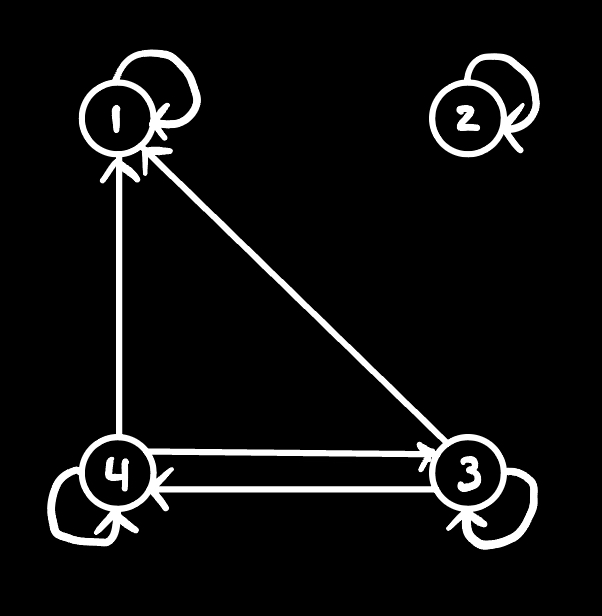
\includegraphics[width = 0.25\textwidth]{./Images/P2-Graph.jpg}
        \end{center}
    \end{Highlight}

    \begin{Highlight}[Solution - Part (b)]
        \begin{itemize}
            \item \textbf{Reflexive:} Each element in this graph is related to itself, this relation \textbf{is reflexive}. We have $(1,1), (2,2), (3,3), (4,4)$.
            \item \textbf{Symmetric:} Only elements 3 and 4 depict symmetry, this relation \textbf{is not symmetric}. For example, we have $(3,4)$ and $(4,3)$, $(3,1)$ but not $(1,3)$, etc.
            \item \textbf{Transitive:} Not every element depicts transitivity, this relation \textbf{is not transitive}. For example, we have $(3,4), (4,1), (3,1)$ but not $(1,2),(2,3),(1,3)$.
            \item \textbf{Equivalence:} Since this relation is only reflexive, this relation \textbf{is not an equivalence relation}.
        \end{itemize}
    \end{Highlight}

    \begin{Highlight}[Solution - Part (c)]
        \begin{enumerate}[label = (\arabic*)]
            \item The complement $\bar{R}$ for our relation $R$ is
            \setcounter{equation}{0}
            \footnotesize{
                \begin{align}
                    A \times A & = \{(1,1),(1,2),(1,3),(1,4),(2,1),(2,2),(2,3),(2,4),(3,1),(3,2),(3,3),(3,4),(4,1),(4,2),(4,3),(4,4)\} \\
                    \bar{R} & = (A \times A) - R = \{(1,2),(1,3),(1,4),(2,1),(2,3),(2,4),(3,2),(4,2)\}
                \end{align}
            }
            \normalsize
            \item The complement $\bar{R}$ consists of all the pairs that are not present in $R$. A relation can be symmetric, and the complement of that relation can not be symmetric. Because the
            complement is the pairs that are not present in the original relation, we can create a complement such that all its pairs are not symmetric. So this statement is \textbf{false}.
        \end{enumerate}
    \end{Highlight}
\end{problem}

% Problem 3
\begin{problem}{Problem 3}
    \begin{statement}{Problem Statement}
        Do the proof of example 3 on page 609 in your OWN WORDS AND METHODS. You can make this more straightforward I believe. Notice the “if and only if” elements. You may use Definition and Theorems 
        from page 240-241.
    \end{statement}

    \begin{Highlight}[Solution]
        \noindent \textbf{Theorem:} $R = \{(a,b) | a \equiv b \hspace*{1pt} (\hspace*{-3pt} \modulo m)\}$ is an equivalence relation. \vspace*{1em}

        \noindent \textbf{Direct Proof:}
        \begin{align*}
            \text{There exists integers } a, b, m \text{ such that } a & \equiv b \modulo m & \text{(Premise)} \\
            \text{Integer } b & = a & \text{(Closure)} \\
            \text{There exists an integer } k \text{ such that } a - a & = km & \text{(Theorem 4)} \\
            a & \equiv a \modulo m & \text{(Definition Of Congruence)} \\
            \text{Therefore we can say congruence modulo } m & \text{ is reflexive} & \text{(Reflexive Congruence)} \\
            \text{Integer } b & \neq a & \text{(Closure)} \\
            \text{There exists an integer } k \text{ such that } a - b & = km & \text{(Theorem 4)} \\
            a & \equiv b \modulo m & \text{(Definition Of Congruence)} \\
            \text{There exists an integer } k \text{ such that } b - a & = (-k)m & \text{(Theorem 4)} \\
            b & \equiv a \modulo m & \text{(Definition Of Congruence)} \\
            \text{Therefore we can say congruence modulo } m & \text{ is symmetric} & \text{(Symmetric Congruence)} \\
            \text{There exists integers } a, b, m \text{ such that } a & \equiv b \modulo m & \text{(Premise)} \\
            \text{There exists an integer } k \text{ such that } a - b & = km & \text{(Theorem 4)} \\
            a & = b + km & \text{(Algebra)} \\
            \text{There exists integers } b, c, m \text{ such that } b & \equiv c \modulo m & \text{(Premise)} \\
            \text{There exists an integer } l \text{ such that } b - c & = lm & \text{(Theorem 4)} \\
            c & = b - lm & \text{(Algebra)} \\
            a - c & = b + km - (b - lm) & \text{(Substitution)} \\
            & = \cancel{b} + km - \cancel{b} + lm & \text{(Simplification)} \\
            & = (k + l)m & \text{(Factoring)} \\
            \text{Let integer } \alpha & = (k + l) & \text{(Closure)} \\
            a - c & = \alpha m & \text{(Substitution)} \\
            a & \equiv c \modulo m & \text{(Definition Of Congruence)} \\
            \text{Therefore we can say congruence modulo } m & \text{ is transitive} & \text{(Transitive Congruence)}
        \end{align*}
        Consequently, from the above, we can see that that the relation $R$ is reflexive, symmetric, and transitive and therefore an equivalence relation. \qed
    \end{Highlight}
\end{problem}